\clearpage
\phantomsection

\setcounter{chapter}{3}
\chapter[{KẾT QUẢ THỰC NGHIỆM VÀ ĐÁNH GIÁ}]{Kết quả thực nghiệm và đánh giá}

Chương này trình bày kết quả thực nghiệm trên CombatAgent. Khác với kết quả ban đầu chỉ gồm một run ngắn 200 nghìn bước, bộ thí nghiệm cuối cùng gồm nhiều run từ 1 triệu đến 3 triệu bước, tập trung vào các yếu tố: phần thưởng nội tại, LSTM, curriculum learning, giảm phương sai vị trí sinh và thiết kế lại phần thưởng. Trong phạm vi các run đã thực hiện, curriculum learning là xu hướng cải thiện nổi bật nhất; ICM chỉ tạo khác biệt rõ khi được ghép sau curriculum, còn các kỹ thuật còn lại chủ yếu dao động quanh cùng một mức trần hiệu năng.

\section{Chỉ số đánh giá}

Các scalar được trích từ log huấn luyện TensorBoard và tổng hợp thành các bảng chỉ số phục vụ phân tích. Bảng~\ref{tab:tensorboard_metrics} trình bày các chỉ số được dùng trong phần này.

Do ngân sách huấn luyện không hoàn toàn đồng nhất giữa nhóm không curriculum và nhóm curriculum, các so sánh giữa hai nhóm được hiểu là so sánh giữa các cấu hình huấn luyện hoàn chỉnh, không phải kiểm định cô lập tuyệt đối tác động của riêng curriculum. Cụ thể, run34, run35, run36 và run42 dừng ở 1.0M bước, trong khi các run curriculum chính chạy đến 3.0M bước; hạn chế này được nhắc lại ở phần tổng hợp kết quả.
\begin{table}[H]
    \centering
    \small
    \setlength{\tabcolsep}{4pt}
    \renewcommand{\arraystretch}{1.25}
    \caption{Các chỉ số TensorBoard dùng trong phân tích}
    \label{tab:tensorboard_metrics}
    \begin{tabular}{|>{\raggedright\arraybackslash}p{3.4cm}|>{\raggedright\arraybackslash}p{6.2cm}|>{\raggedright\arraybackslash}p{6.2cm}|}
        \hline
        \textbf{Nhóm chỉ số} & \textbf{Cột trong CSV} & \textbf{Ý nghĩa sử dụng} \\
        \hline
        Bước huấn luyện & last\_step & Số bước môi trường cuối cùng được ghi nhận trong event file, dùng để kiểm tra độ dài run. \\
        \hline
        Reward chính & reward\_tail50, reward\_hard\_from\_140k & Reward cuối run và reward trung bình sau khi curriculum đã vào Hard; dùng để so sánh hiệu năng thay vì chỉ nhìn peak. \\
        \hline
        Hành vi combat & kills\_tail50, cleared\_tail50, damage\_dealt\_tail50, damage\_taken\_tail50 & Cho biết agent thật sự tiêu diệt địch, dọn phòng và trao đổi sát thương ra sao, tránh diễn giải reward tổng hợp một cách mơ hồ. \\
        \hline
        Dash & useful\_dash\_rate\_tail50, wasteful\_dash\_rate\_tail50, dash\_actions\_per\_decision\_tail50, blocked\_dash\_actions\_per\_decision\_tail50 & Đánh giá agent có dùng dash như một kỹ năng chiến đấu hay chỉ gần như không dùng/không bị mask. \\
        \hline
        Policy & entropy\_tail50, extrinsic\_value\_estimate\_tail50 & Entropy đo mức stochastic của policy; value estimate cho biết critic đang đặt kỳ vọng extrinsic reward ở mức nào. \\
        \hline
        Loss & policy\_loss\_tail50, value\_loss\_tail50, icm\_inverse\_loss\_tail50 & Theo dõi độ ổn định cập nhật PPO và chất lượng representation của ICM. \\
        \hline
        Intrinsic reward & curiosity\_reward\_tail50, rnd\_reward\_tail50 & Phần thưởng nội tại của ICM/RND, dùng để đọc riêng đóng góp của curiosity. \\
        \hline
        Reward trung bình trượt & rolling reward 200k bước & Reward được làm mượt theo cửa sổ 200 nghìn bước, dùng để vẽ biểu đồ xu hướng học thay vì chỉ nhìn một điểm cuối. \\
        \hline
    \end{tabular}
\end{table}

Với các run curriculum, khóa luận ưu tiên reward mean trên vùng Hard từ sau bước 140 nghìn và các chỉ số hành vi ở tail-50 cuối run. Các cột peak, head/tail chi tiết hoặc mốc Hard phụ chỉ được dùng khi cần giải thích một hiện tượng cụ thể, vì bảng chính cần phản ánh năng lực combat và trạng thái học của policy hơn là ghi lại quá nhiều số log.

\begin{table}[H]
    \centering
    \scriptsize
    \setlength{\tabcolsep}{4pt}
    \renewcommand{\arraystretch}{1.15}
    \caption{Các chỉ số hành vi chính ở cuối quá trình huấn luyện}
    \label{tab:run_metrics_main}
    \begin{tabular}{l p{3.0cm} c c c c c c c c}
        \toprule
        \textbf{Run} & \textbf{Thiết lập} & \textbf{Step} & \textbf{Reward} & \textbf{Clear} & \textbf{Kills} & \textbf{Dmg+} & \textbf{Dmg-} & \textbf{Dash+} & \textbf{Ent} \\
        \midrule
        run34 & PPO baseline & 1.00M & 2.073 & 0.129 & 0.721 & 25.977 & 16.867 & 0.149 & 4.408 \\
        run35 & PPO + ICM & 1.00M & 2.416 & 0.173 & 0.752 & 26.614 & 15.242 & 0.116 & 4.407 \\
        run36 & PPO + RND & 1.00M & 2.487 & 0.159 & 0.796 & 28.068 & 14.013 & 0.107 & 4.406 \\
        run42 & PPO + LSTM & 1.00M & 2.411 & 0.163 & 0.769 & 27.140 & 15.775 & 0.132 & 4.405 \\
        run46 & PPO + Curriculum & 3.00M & 3.843 & 0.267 & 0.994 & 35.135 & 19.368 & 0.245 & 4.409 \\
        run47 & Curriculum + LSTM & 3.00M & 3.765 & 0.241 & 0.921 & 32.884 & 16.420 & 0.228 & 4.405 \\
        run50 & Curriculum + ICM & 3.00M & 4.369 & 0.273 & 1.016 & 36.161 & 23.132 & 0.334 & 4.411 \\
        run54 & 4-tier fixed-to-random & 3.00M & 3.925 & 0.242 & 0.945 & 33.673 & 17.966 & 0.179 & 4.407 \\
        run55 & Curriculum + reward v2 & 3.00M & 9.337 & 0.267 & 1.014 & 35.685 & 21.312 & 0.240 & 4.407 \\
        \bottomrule
    \end{tabular}
\end{table}

\begin{table}[H]
    \centering
    \scriptsize
    \setlength{\tabcolsep}{5pt}
    \renewcommand{\arraystretch}{1.15}
    \caption{Các chỉ số loss, policy và intrinsic reward}
    \label{tab:run_metrics_aux}
    \begin{tabular}{l p{3.5cm} c c c c c c}
        \toprule
        \textbf{Run} & \textbf{Thiết lập} & \textbf{P-loss} & \textbf{V-loss} & \textbf{V-est} & \textbf{Dash/dec} & \textbf{ICM inv.} & \textbf{Int. rew.} \\
        \midrule
        run34 & PPO baseline & 0.016 & 0.140 & 0.170 & 0.0002 & -- & -- \\
        run35 & PPO + ICM & 0.017 & 0.072 & 0.169 & 0.0002 & 4.360 & 0.150 \\
        run36 & PPO + RND & 0.016 & 0.071 & 0.167 & 0.0002 & -- & 0.099 \\
        run42 & PPO + LSTM & 0.082 & 0.168 & 0.178 & 0.0002 & -- & -- \\
        run46 & PPO + Curriculum & 0.017 & 0.207 & 0.401 & 0.0005 & -- & -- \\
        run47 & Curriculum + LSTM & 0.079 & 0.229 & 0.380 & 0.0004 & -- & -- \\
        run50 & Curriculum + ICM & 0.016 & 0.113 & 0.483 & 0.0011 & 4.337 & 0.185 \\
        run54 & 4-tier fixed-to-random & 0.017 & 0.200 & 0.416 & 0.0005 & -- & -- \\
        run55 & Curriculum + reward v2 & 0.016 & 0.662 & 0.962 & 0.0005 & -- & -- \\
        \bottomrule
    \end{tabular}
\end{table}

Trong Bảng~\ref{tab:run_metrics_main}, Reward là reward\_tail50 với các run không curriculum và reward\_hard\_from\_140k với các run curriculum; Clear, Kills, Dmg+/Dmg-, Dash+ và Ent lần lượt là cleared\_tail50, kills\_tail50, damage\_dealt/taken\_tail50, useful\_dash\_rate\_tail50 và entropy\_tail50. Bảng~\ref{tab:run_metrics_aux} giữ các tín hiệu chẩn đoán quan trọng: policy loss, value loss, extrinsic value estimate, tần suất dash, inverse loss của ICM và intrinsic reward. Các cột trống được ký hiệu ``--'' vì run tương ứng không sử dụng kỹ thuật đó.

\begin{figure}[H]
    \centering
    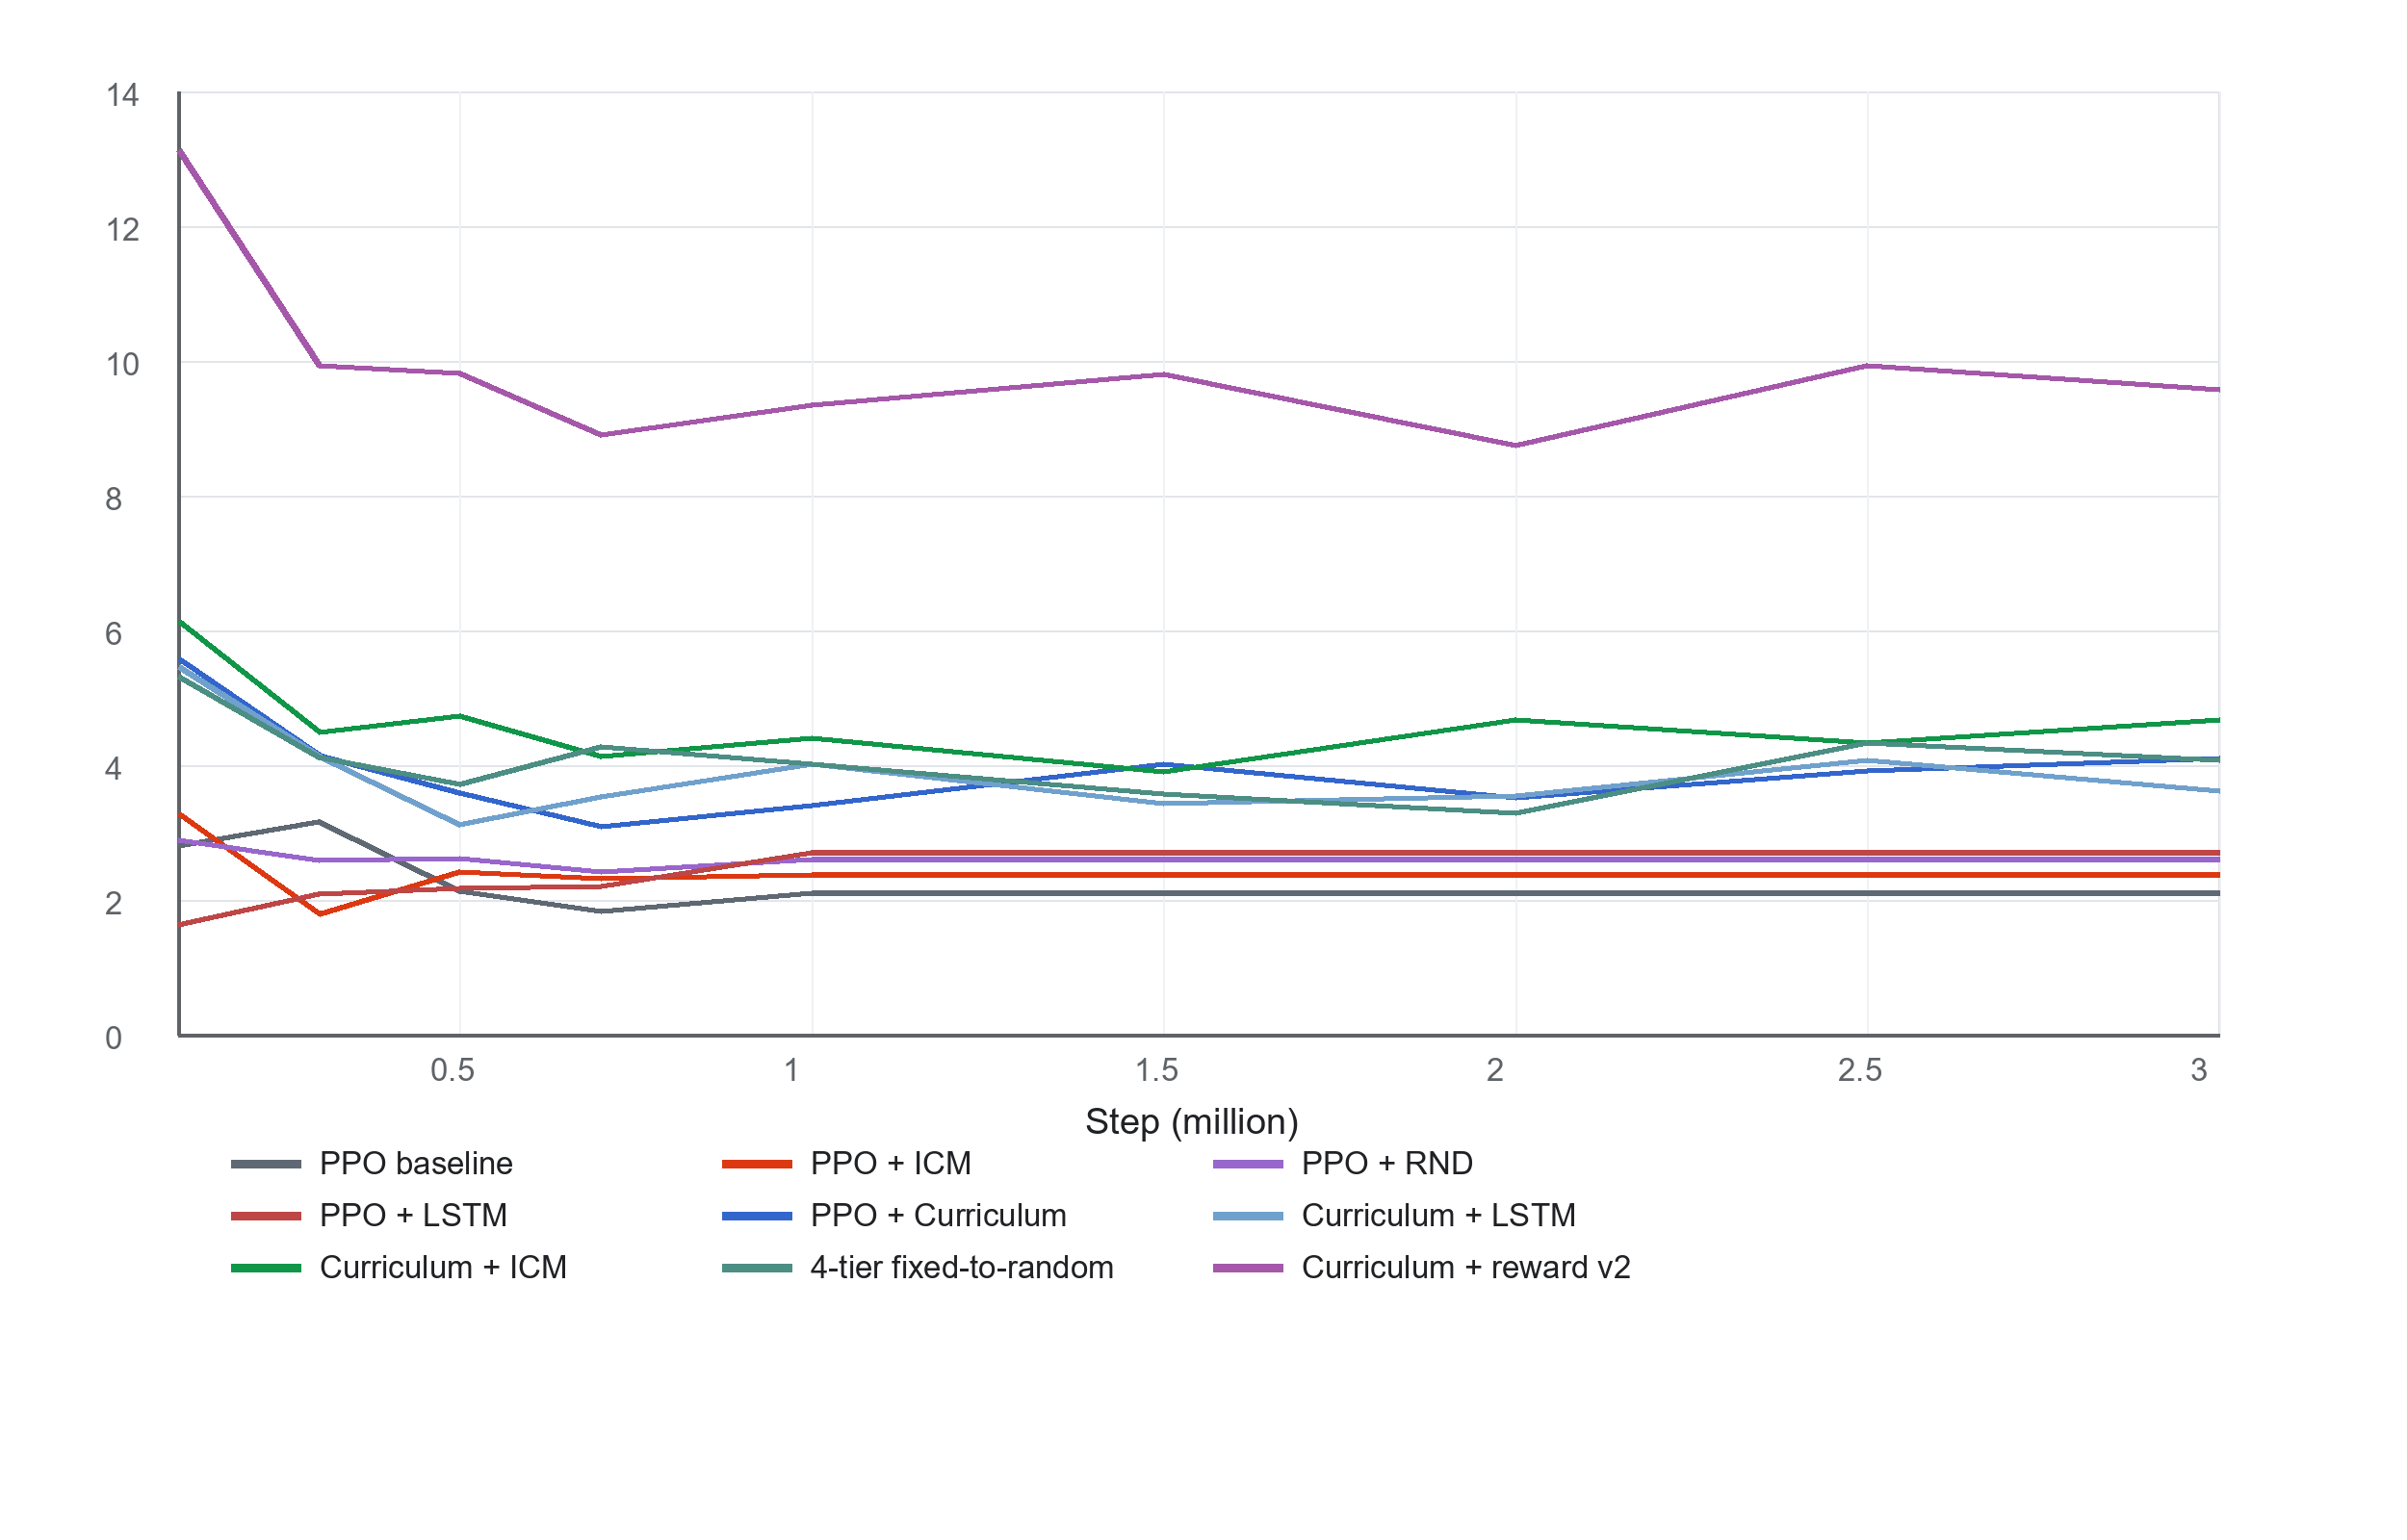
\includegraphics[width=0.98\textwidth]{figures/training/training_reward_curves.png}
    \caption{Đường reward trong quá trình huấn luyện của các cấu hình chính}
    \label{fig:training_reward_curves}
\end{figure}

Các run không dùng curriculum kết thúc ở 1M bước nên được giữ phẳng sau mốc này để thuận tiện so sánh trực quan trên cùng một trục thời gian. Riêng run55 sử dụng reward v2, do đó giá trị reward tuyệt đối của run này không được so trực tiếp với các run dùng reward v1; hình chủ yếu dùng để đọc xu hướng học và vị trí tương đối giữa các nhóm thí nghiệm.

\section{PPO nền và các phần thưởng nội tại}

Run34 là cấu hình PPO nền, chưa áp dụng curriculum learning. Sau 1 triệu bước huấn luyện, reward tích lũy trung bình trên 50 episode cuối đạt 2.073, tỷ lệ dọn phòng trung bình đạt 0.129 và tỷ lệ dọn phòng cao nhất đạt 0.50. Kết quả này cho thấy tác nhân đã học được một số hành vi cơ bản như tiếp cận và tấn công kẻ địch, nhưng chưa duy trì ổn định khả năng dọn phòng trên phân phối bản đồ khó.

Hai biến thể phần thưởng nội tại được đánh giá là ICM ở run35 và RND ở run36. ICM đạt reward tail-50 là 2.416, trong khi RND đạt 2.487. Mặc dù cả hai đều cải thiện so với PPO nền, mức tăng còn tương đối nhỏ và chưa tạo ra thay đổi bản chất trong hành vi của tác nhân. Điều này gợi ý rằng khó khăn chính của môi trường không chỉ nằm ở việc thiếu tín hiệu khám phá, mà còn đến từ độ khó ban đầu của phân phối bản đồ và nhiệm vụ chiến đấu.

\begin{figure}[H]
    \centering
    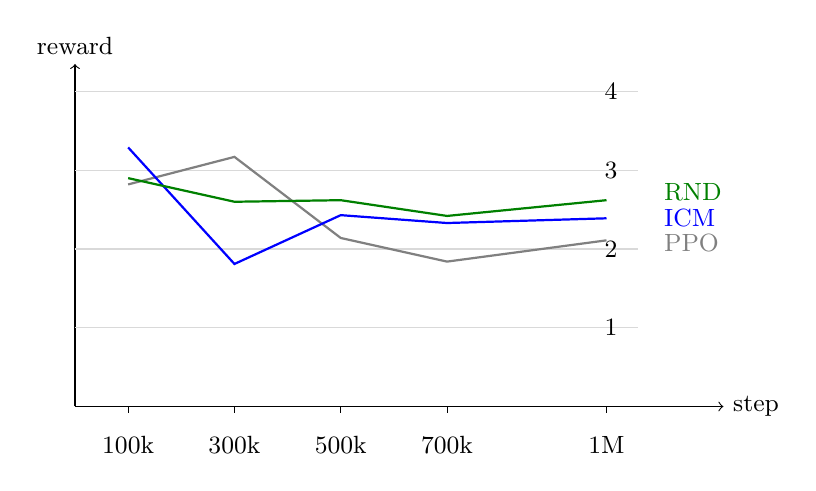
\begin{tikzpicture}[x=1.35cm,y=1.0cm, every node/.style={font=\small}]
        \draw[->] (0,0) -- (6.1,0) node[right]{step};
        \draw[->] (0,0) -- (0,4.35) node[above]{reward};
        
        \foreach \y in {1,2,3,4}
            \draw[gray!30] (0,\y) -- (5.3,\y) node[left=4pt, black]{\y};
        
        \foreach \x/\label in {0.5/100k,1.5/300k,2.5/500k,3.5/700k,5.0/1M}
            \draw (\x,0) -- (\x,-0.08) node[below=5pt]{\label};
        
        \draw[thick, gray] plot coordinates {
            (0.5,2.82) (1.5,3.17) (2.5,2.14) (3.5,1.84) (5.0,2.11)
        };
        \draw[thick, blue] plot coordinates {
            (0.5,3.29) (1.5,1.81) (2.5,2.43) (3.5,2.33) (5.0,2.39)
        };
        \draw[thick, green!50!black] plot coordinates {
            (0.5,2.90) (1.5,2.60) (2.5,2.62) (3.5,2.42) (5.0,2.62)
        };
        
        % Labels: đẩy sang phải và tách dọc để không dính nhau
        \node[green!50!black, anchor=west] at (5.45,2.72){RND};
        \node[blue, anchor=west] at (5.45,2.40){ICM};
        \node[gray, anchor=west] at (5.45,2.08){PPO};
    \end{tikzpicture}
    \caption{Rolling mean reward 200k bước của PPO baseline, ICM và RND trong 1M bước đầu}
    \label{fig:baseline_intrinsic_reward}
\end{figure}

\subsection{ICM và dấu hiệu encoding collapse}

ICM học một inverse model dự đoán hành động từ trạng thái trước và sau \cite{Pathak2017}. Với action space $(3,3,3,9)$, entropy ngẫu nhiên lý thuyết là khoảng 5.49 nat. Inverse loss của run35 quanh 4.36, chỉ giảm khoảng 21\% so với mức ngẫu nhiên lý thuyết. Điều này cho thấy encoding học được còn yếu: representation không phân biệt tốt tác động của từng nhánh hành động trong môi trường nhiều yếu tố nhiễu như đạn, kẻ địch và procedural map.

\begin{figure}[H]
    \centering
    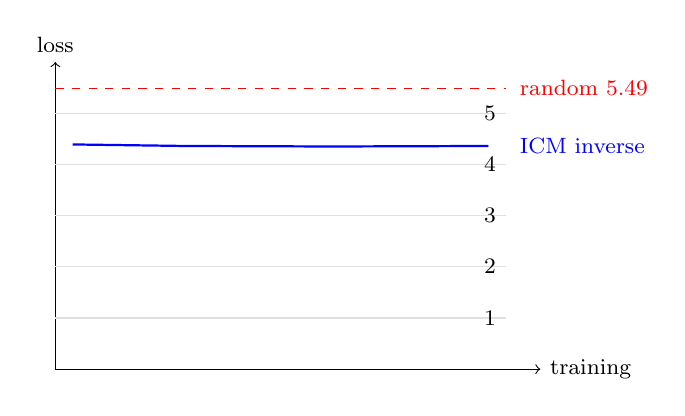
\begin{tikzpicture}[x=1.1cm,y=0.65cm, every node/.style={font=\footnotesize}]
        \draw[->] (0,0) -- (5.6,0) node[right]{training};
        \draw[->] (0,0) -- (0,6.0) node[above]{loss};
        \foreach \y/\label in {1/1,2/2,3/3,4/4,5/5} \draw[gray!25] (0,\y) -- (5.2,\y) node[left, black]{\label};
        \draw[dashed, red] (0,5.49) -- (5.2,5.49);
        \node[red, anchor=west] at (5.25,5.49){random 5.49};
        \draw[thick, blue] plot coordinates {(0.2,4.39) (1.5,4.36) (3.2,4.35) (5.0,4.36)};
        \node[blue, anchor=west] at (5.25,4.36){ICM inverse};
    \end{tikzpicture}
    \caption{Inverse loss của ICM duy trì gần mức ngẫu nhiên lý thuyết}
    \label{fig:icm_inverse_plateau}
\end{figure}

RND không cần dự đoán hành động nên tránh được inverse loss collapse \cite{Burda2018}, nhưng reward nội tại của run36 giảm nhanh về mức nhỏ khi model dự đoán quen với phân phối quan sát. Vì vậy, RND tốt hơn ICM một chút ở reward tail-50, nhưng vẫn chưa vượt qua trần baseline một cách đáng kể.

\section{Ảnh hưởng của LSTM}

Run42 thêm LSTM với bộ nhớ kích thước 256 và chuỗi quan sát dài 64 bước. Khác với ICM/RND, LSTM có xu hướng học chậm nhưng tăng dần về cuối. Rolling reward 200k bước tăng từ 1.64 ở mốc 100k lên 2.71 ở mốc 1M. Điều này phù hợp với giả thuyết rằng bộ nhớ có ích cho hồi chiêu, đạn và trạng thái khuất tầm nhìn, nhưng lợi ích chưa đủ lớn để tạo thay đổi nổi bật trong ngân sách huấn luyện hiện tại.

\begin{figure}[H]
    \centering
    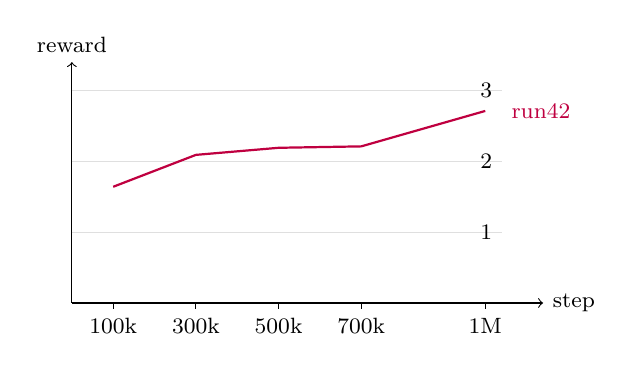
\begin{tikzpicture}[x=1.05cm,y=0.9cm, every node/.style={font=\footnotesize}]
        \draw[->] (0,0) -- (5.7,0) node[right]{step};
        \draw[->] (0,0) -- (0,3.4) node[above]{reward};
        \foreach \y in {1,2,3} \draw[gray!25] (0,\y) -- (5.2,\y) node[left, black]{\y};
        \foreach \x/\label in {0.5/100k,1.5/300k,2.5/500k,3.5/700k,5.0/1M}
            \draw (\x,0) -- (\x,-0.08) node[below]{\label};
        \draw[thick, purple] plot coordinates {(0.5,1.64) (1.5,2.09) (2.5,2.19) (3.5,2.21) (5.0,2.71)};
        \node[purple, anchor=west] at (5.2,2.71){run42};
    \end{tikzpicture}
    \caption{Run42 LSTM-only có xu hướng tăng dần nhưng vẫn quanh mức intrinsic reward}
    \label{fig:lstm_trend}
\end{figure}

Kết quả này cho thấy memory architecture có thể là hướng cải tiến phụ, nhưng không giải quyết vấn đề chính của môi trường: agent vẫn bắt đầu từ phân phối Hard quá rộng và khó nhận được chuỗi reward thành công đủ thường xuyên.

\section{curriculum learning: cải thiện nổi bật}

Run46 là thí nghiệm quan trọng nhất. Curriculum bắt đầu ở Easy, chuyển sang Medium tại khoảng 70k bước và chuyển sang Hard tại khoảng 140k bước. Sau khi vào Hard, reward mean đạt 3.843, cao hơn 85\% so với baseline tail-50 2.073:

\begin{equation}
    \frac{3.843 - 2.073}{2.073} \approx 85\%.
\end{equation}

\begin{figure}[H]
    \centering
    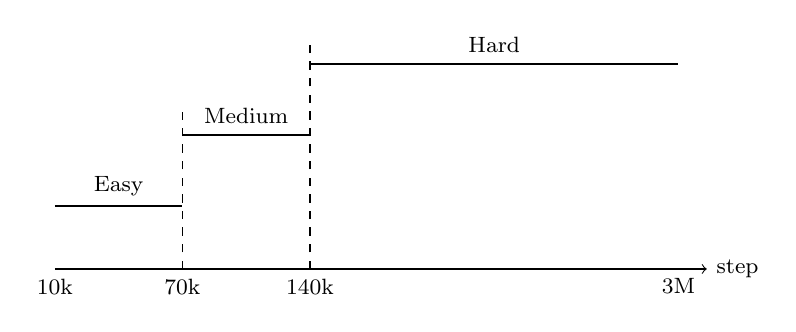
\begin{tikzpicture}[x=0.9cm,y=1cm, every node/.style={font=\footnotesize}]
        \draw[->] (0,0) -- (9.2,0) node[right]{step};
        \draw[thick] (0,0.8) -- (1.8,0.8);
        \draw[thick] (1.8,1.7) -- (3.6,1.7);
        \draw[thick] (3.6,2.6) -- (8.8,2.6);
        \draw[dashed] (1.8,0) -- (1.8,2.0);
        \draw[dashed] (3.6,0) -- (3.6,2.9);
        \node at (0.9,1.05){Easy};
        \node at (2.7,1.95){Medium};
        \node at (6.2,2.85){Hard};
        \node[below] at (0,0){10k};
        \node[below] at (1.8,0){70k};
        \node[below] at (3.6,0){140k};
        \node[below] at (8.8,0){3M};
    \end{tikzpicture}
    \caption{Lesson transition của run46: Easy $\rightarrow$ Medium $\rightarrow$ Hard}
    \label{fig:run46_lesson_transition}
\end{figure}

Reward theo lesson của run46 cho thấy Easy mean 6.364, Medium mean 4.181 và Hard mean 3.843. Khi vào Hard, đường reward không tăng tuyến tính mà dao động trong vùng 3.1--4.2 theo rolling window 200k bước. Dao động này là hợp lý vì nhóm Hard có nhiều cấu hình bản đồ hơn, đồng thời spawn và phân phối enemy cũng đa dạng hơn.

\begin{figure}[H]
    \centering
    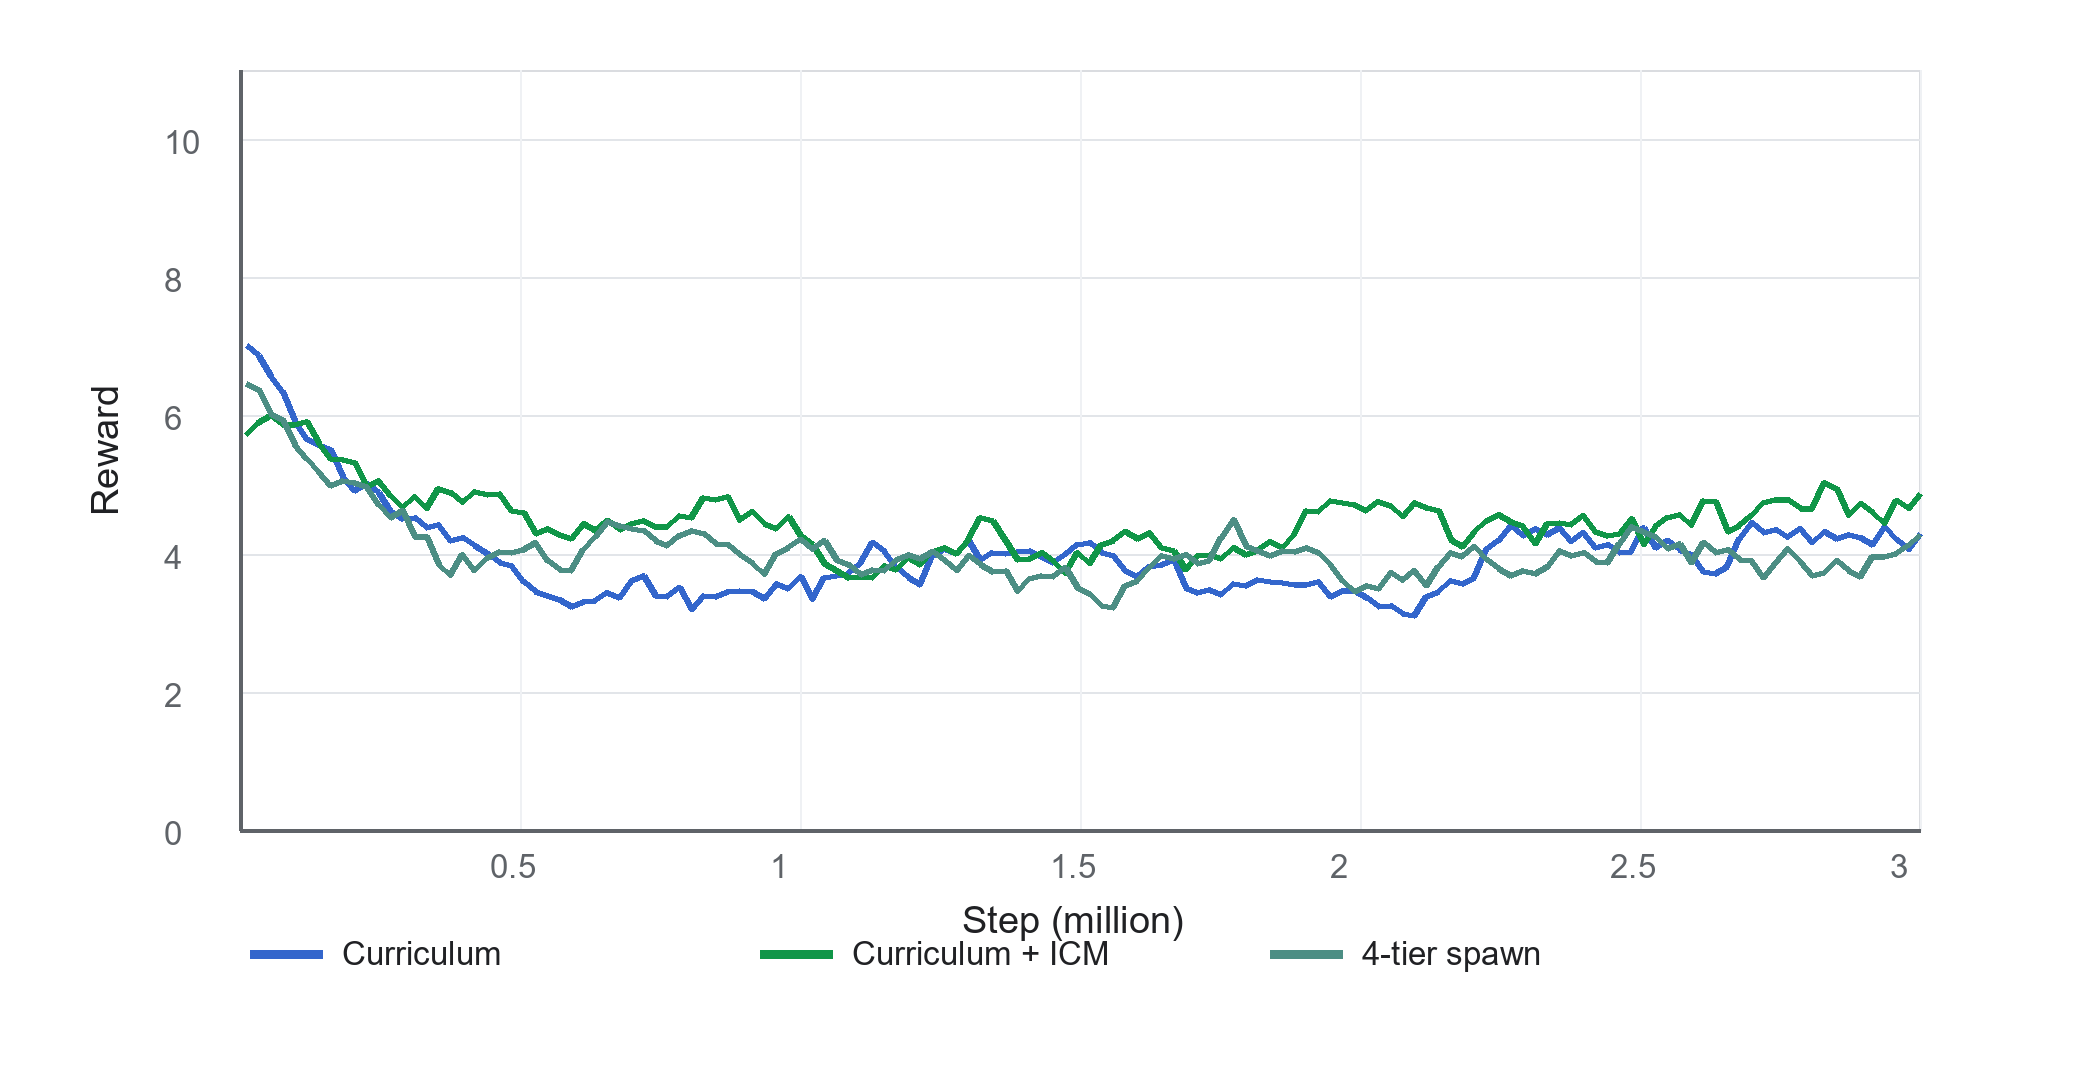
\includegraphics[width=0.98\textwidth]{figures/training/curriculum_reward_trend.png}
    \caption{Xu hướng reward trong các run curriculum}
    \label{fig:curriculum_reward_trend}
    \vspace{0.2em}
    \begin{minipage}{0.94\textwidth}
        \small
        Hình cho thấy reward không tăng đều sau khi vào Hard mà dao động quanh một vùng ổn định. Run50 cao hơn run46 ở phần sau quá trình huấn luyện, gợi ý ICM chỉ phát huy rõ khi policy đã có kỹ năng nền từ curriculum.
    \end{minipage}
\end{figure}

\begin{figure}[H]
    \centering
    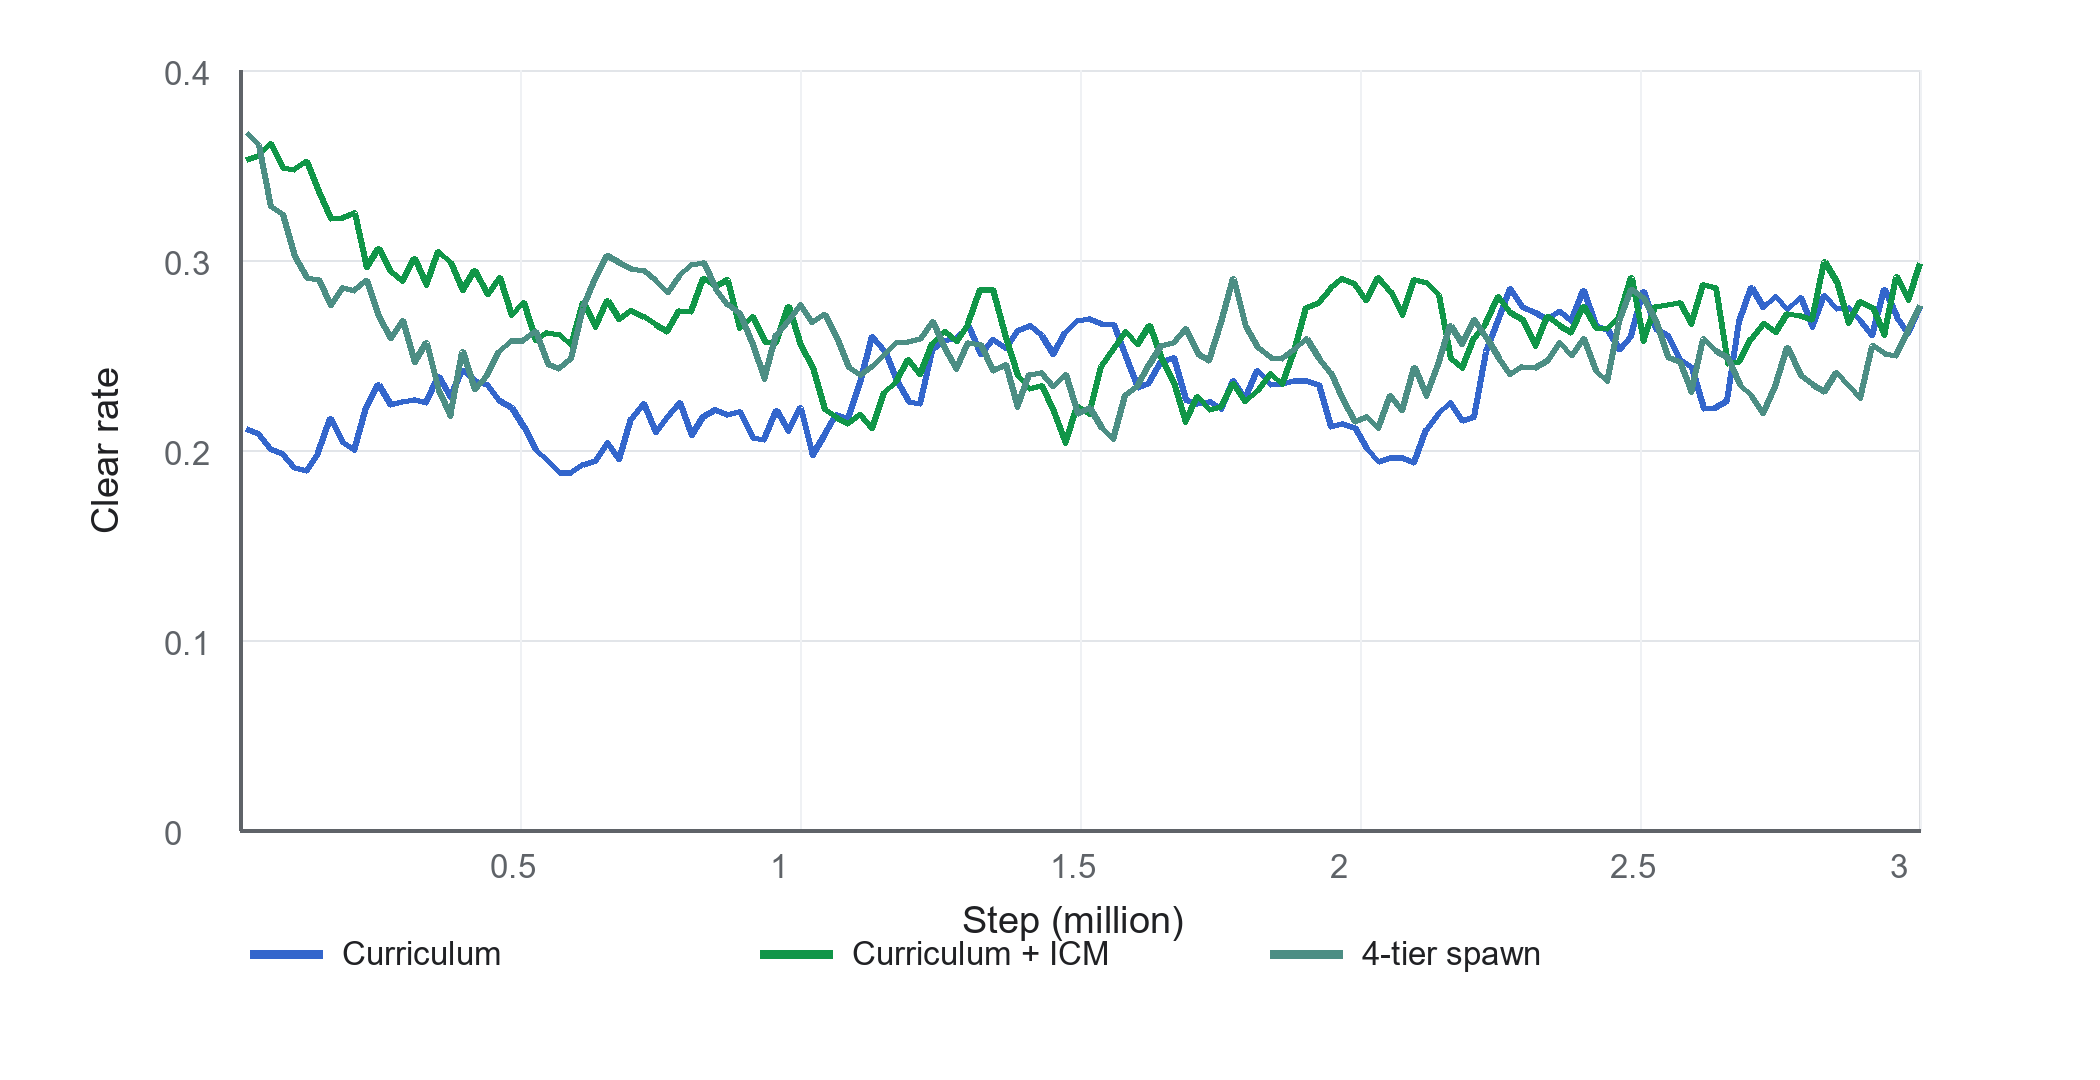
\includegraphics[width=0.98\textwidth]{figures/training/curriculum_clear_rate_trend.png}
    \caption{Xu hướng tỷ lệ dọn phòng trong các run curriculum}
    \label{fig:curriculum_clear_rate_trend}
    \vspace{0.2em}
    \begin{minipage}{0.94\textwidth}
        \small
        Tỷ lệ dọn phòng tăng mạnh ở giai đoạn đầu rồi chững lại khi bài toán chuyển sang phân phối Hard. Vì clear rate là chỉ số outcome, đường cong này bổ sung cho reward bằng cách cho thấy cải thiện không chỉ đến từ shaping reward.
    \end{minipage}
\end{figure}

\begin{figure}[H]
    \centering
    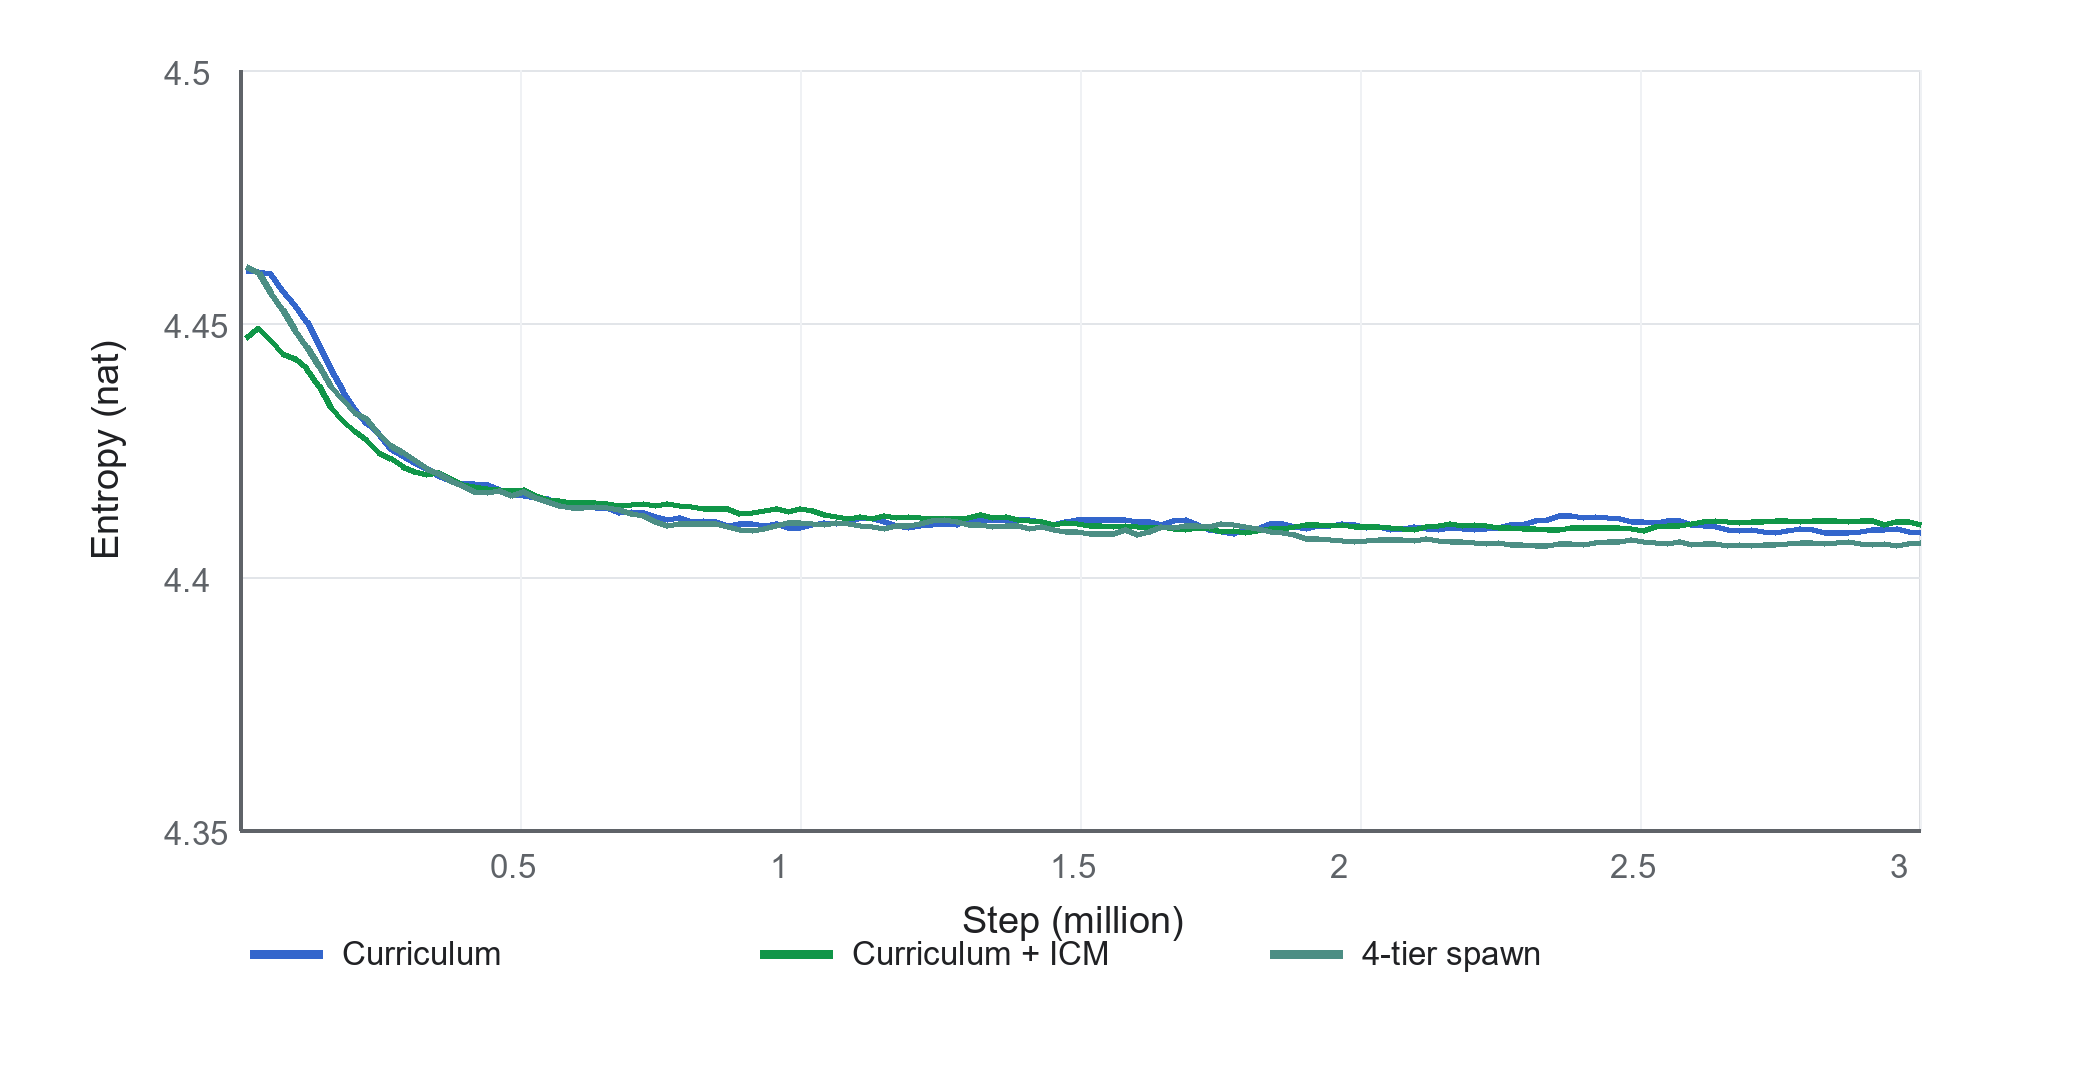
\includegraphics[width=\textwidth]{figures/training/curriculum_entropy_trend.png}
    \caption{Xu hướng entropy policy trong các run curriculum}
    \label{fig:curriculum_entropy_trend}
    \vspace{0.2em}
    \begin{minipage}{0.94\textwidth}
        \small
        Entropy của ba run nhanh chóng rơi về vùng xấp xỉ 4.40 nat và gần như đi ngang. Điều này giải thích vì sao tăng reward/clear rate không đồng nghĩa với việc policy trở nên quyết định hơn đáng kể.
    \end{minipage}
\end{figure}

\begin{figure}[H]
    \centering
    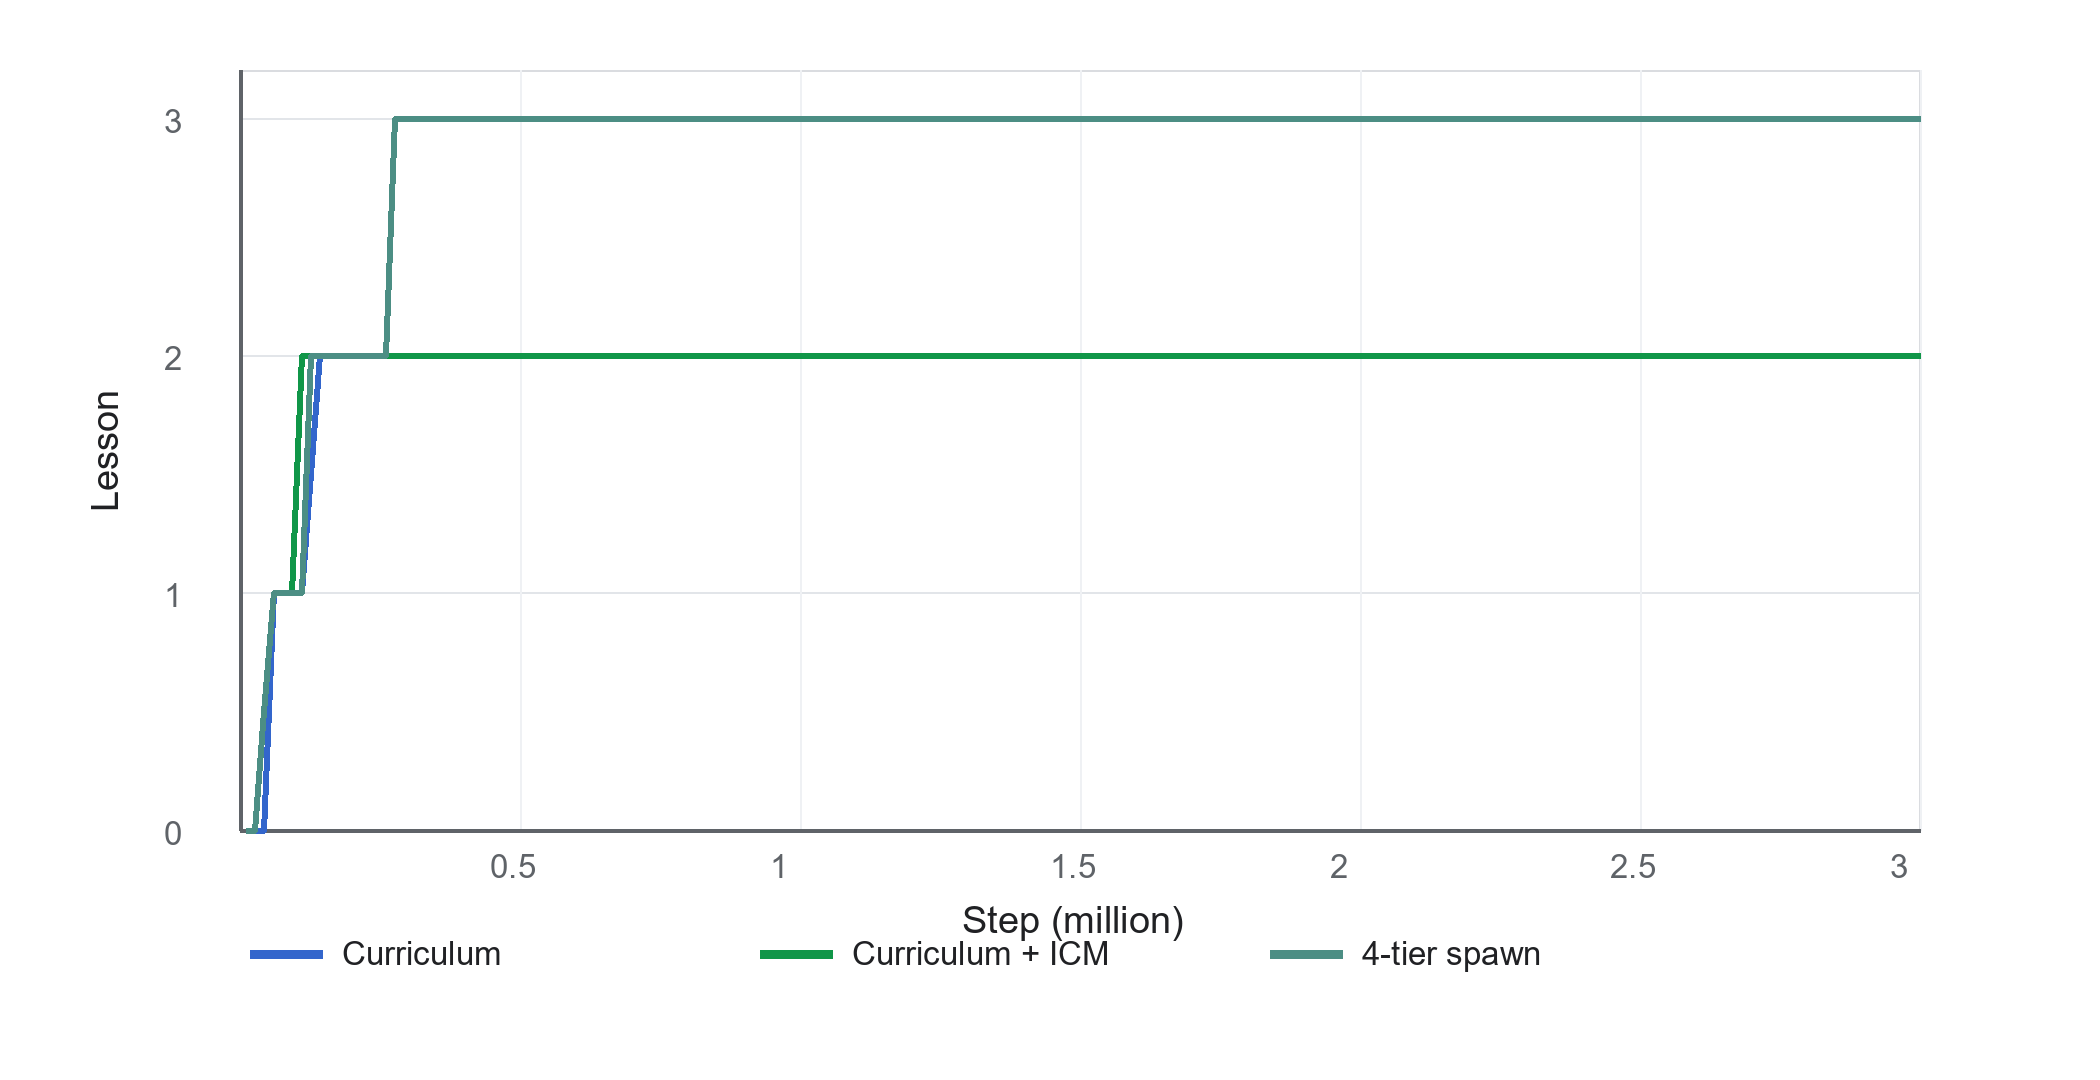
\includegraphics[width=\textwidth]{figures/training/curriculum_lesson_schedule.png}
    \caption{Lịch chuyển lesson trong các run curriculum}
    \label{fig:curriculum_lesson_schedule}
    \vspace{0.2em}
    \begin{minipage}{0.94\textwidth}
        \small
        Run46 và run50 chuyển lên Hard từ rất sớm nên phần lớn 3M bước vẫn đánh giá trên cùng phân phối khó. Run54 có thêm lesson Hard Random, vì vậy đường lesson đạt mức 3 và phản ánh biến thể fixed-to-random spawn.
    \end{minipage}
\end{figure}

Trong phạm vi các run đã thực hiện, đây là xu hướng mạnh nhất của khóa luận: curriculum không chỉ tăng reward trung bình mà còn tăng các chỉ số hành vi. Tail-50 của run46 đạt 0.994 kills/episode và cleared tail-50 đạt 0.267, cao hơn rõ rệt so với baseline. Về mặt cơ chế, curriculum có thể được hiểu như một dạng "giàn giáo gradient": ở Easy, agent gặp các episode thành công đủ thường xuyên để học chuỗi tiếp cận -- ngắm -- tấn công; khi sang Medium và Hard, policy đã có kỹ năng nền thay vì khám phá từ gần như ngẫu nhiên. Tuy nhiên, do mỗi cấu hình mới chỉ có một seed, kết luận này cần được xác nhận thêm bằng các run lặp lại có error bar.

\section{Thử nghiệm kết hợp LSTM và ICM trên nền curriculum learning}

Run47 thêm LSTM vào curriculum. Hard mean đạt 3.765, thấp hơn nhẹ so với 3.843 của run46. Chênh lệch này nhỏ và chưa đủ để kết luận LSTM làm xấu chính sách, nhưng đủ cho thấy memory không tạo thêm cải thiện rõ ràng khi curriculum đã cung cấp scaffold khám phá.

Có hai giả thuyết giải thích kết quả này. Thứ nhất, \textit{LSTM làm chậm tốc độ hội tụ của PPO}: policy loss của run47 là 0.079, cao hơn gần 5 lần so với run46 là 0.017. Điều này gợi ý rằng các trọng số hồi tiếp của LSTM cần nhiều mẫu hơn để ổn định, khiến policy update kém hiệu quả hơn trong cùng 3M bước. Thứ hai, \textit{curriculum đã giải quyết phần lớn nhu cầu về bộ nhớ}: trong môi trường thưa thưởng, lợi ích chính của LSTM là giúp agent nhớ chuỗi hành vi thành công trong episode dài. Tuy nhiên, khi curriculum đã thu hẹp phân phối bản đồ về Easy/Medium ở giai đoạn đầu, độ dài hiệu quả của chuỗi quyết định ngắn lại, làm giảm lợi thế tương đối của LSTM so với MLP thuần.

Run50 bổ sung ICM trên nền curriculum và được huấn luyện đủ 3.00M bước. Trên vùng Hard, reward mean đạt 4.369, cao hơn run46 là 3.843; tail-50 cuối run đạt 4.707. Một số chỉ số hành vi cũng cải thiện nhẹ, gồm số kẻ địch tiêu diệt trung bình đạt 1.016, cleared tail-50 đạt 0.273 và useful dash rate đạt 0.334. Điều này cho thấy ICM có thể hỗ trợ agent khám phá thêm các hành vi có ích khi đã được curriculum dẫn qua giai đoạn học ban đầu. Tuy nhiên, inverse loss vẫn ở mức cao, khoảng 4.337, chỉ giảm nhẹ so với run35. Do đó, cải thiện của run50 chủ yếu thể hiện ở hành vi và reward, trong khi ICM chưa cho thấy khả năng giải quyết triệt để khó khăn biểu diễn phát sinh từ action space rời rạc nhiều nhánh.

\begin{table}[H]
    \centering
    \small
    \caption{So sánh các stacking test với curriculum baseline}
    \label{tab:stacking_tests}
    \begin{tabular}{|p{4.4cm}|c|c|p{4.8cm}|}
        \hline
        \textbf{Run} & \textbf{Steps log} & \textbf{Reward Hard mean} & \textbf{Nhận xét} \\
        \hline
        run46 Curriculum & 3.0M & 3.843 & Baseline curriculum, cải thiện chính. \\
        \hline
        run47 Curriculum + LSTM & 3.0M & 3.765 & Gần tương đương, không có cộng hưởng rõ. \\
        \hline
        run50 Curriculum + ICM & 3.0M & 4.369 & Cải thiện reward và kill so với run46; inverse loss vẫn cao. \\
        \hline
    \end{tabular}
\end{table}

Kết quả cập nhật này làm kết luận tinh tế hơn: curriculum vẫn là yếu tố nền quan trọng nhất, nhưng ICM có thể tạo thêm lợi ích khi agent đã có kỹ năng nền từ các lesson dễ hơn. Dù vậy, inverse loss còn cao cho thấy curiosity signal chủ yếu hỗ trợ khám phá/hành vi ở mức thực nghiệm, chưa chứng minh rằng representation của ICM đã học tốt quan hệ hành động--chuyển trạng thái trong môi trường này.

\section{Giảm phương sai môi trường bằng spawn cố định rồi ngẫu nhiên}

Run54 mở rộng curriculum thành 4 lesson: Easy Fixed, Medium Fixed, Hard Fixed và Hard Random. Lesson Hard Random bắt đầu khoảng 280k bước. Reward Hard mean đạt 3.925, số kill cuối run đạt 0.945 và damage gây ra đạt 33.673. Các chỉ số này gần run46 nhưng không vượt rõ, nên kết quả này được xem là tie có cải thiện marginal.

\begin{figure}[H]
    \centering
    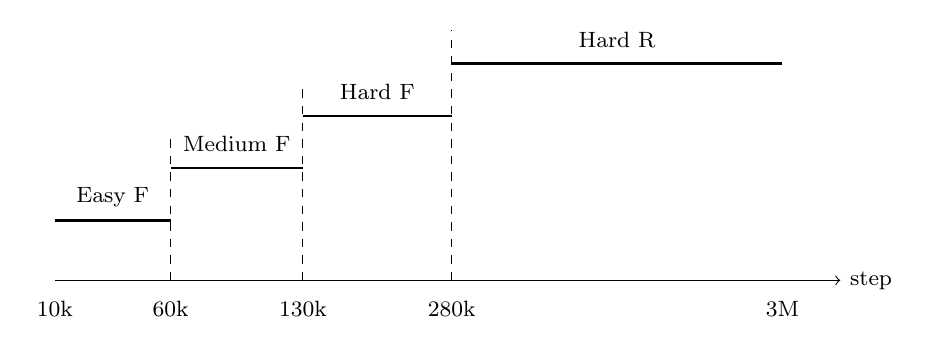
\begin{tikzpicture}[
        x=1.05cm,
        y=0.95cm,
        every node/.style={font=\footnotesize},
        labelnode/.style={fill=white, inner sep=1.5pt}
    ]
        % Axis
        \draw[->] (0,0) -- (9.5,0) node[right]{step};

        % Curriculum tiers
        \draw[thick] (0,0.8) -- (1.4,0.8);
        \draw[thick] (1.4,1.5) -- (3.0,1.5);
        \draw[thick] (3.0,2.2) -- (4.8,2.2);
        \draw[thick] (4.8,2.9) -- (8.8,2.9);

        % Transition markers
        \draw[dashed] (1.4,0) -- (1.4,1.95);
        \draw[dashed] (3.0,0) -- (3.0,2.65);
        \draw[dashed] (4.8,0) -- (4.8,3.35);

        % Labels above each segment
        \node[labelnode] at (0.7,1.12){Easy F};
        \node[labelnode] at (2.2,1.82){Medium F};
        \node[labelnode] at (3.9,2.52){Hard F};
        \node[labelnode] at (6.8,3.22){Hard R};

        % Step labels
        \node[below=4pt] at (0,0){10k};
        \node[below=4pt] at (1.4,0){60k};
        \node[below=4pt] at (3.0,0){130k};
        \node[below=4pt] at (4.8,0){280k};
        \node[below=4pt] at (8.8,0){3M};
    \end{tikzpicture}
    \caption{Curriculum 4-tier của run54: fixed spawn trước, random spawn sau}
    \label{fig:run54_four_tier}
\end{figure}

Fixed spawn giúp giảm phương sai ở giai đoạn đầu, nhưng khi chuyển sang Hard Random thì agent vẫn phải xử lý cùng phân phối khó. Vì vậy, run54 chỉ cải thiện nhẹ ở hành vi combat và không làm thay đổi xu hướng tổng quát: curriculum là yếu tố chính trong nhóm thí nghiệm này, còn fixed-to-random là một biến thể thiết kế môi trường có tác động nhỏ hơn so với chính curriculum.

\section{Reward v2: tăng phần thưởng kết quả nhưng thay đổi thang đo}

Run55 thay đổi reward landscape: tăng mạnh reward kill/clear/damage/aligned attack, giảm reward tiếp cận và phạt idle gần địch mạnh hơn. Log cuối cùng đã đạt 3.00M bước. Reward tail-50 đạt 9.600 và Hard mean đạt 9.337, nhưng không thể so trực tiếp với run46 vì thang reward đã thay đổi.

Chỉ số đáng chú ý hơn là cleared peak đạt 0.80, cao hơn peak 0.615 của run46. Điều này cho thấy outcome-heavy reward có thể đẩy agent tấn công quyết đoán hơn. Tuy nhiên entropy tail vẫn quanh 4.408, nghĩa là reward v2 chưa phá được entropy plateau.

Do đó, run55 được tách khỏi nhóm so sánh reward v1 khi diễn giải reward mean. Với reward v2, các chỉ số đáng dùng hơn là cleared rate, kills, damage gây ra, damage nhận vào, survival hoặc các metric đã chuẩn hóa theo cùng thang đo. Cách tách này tránh việc hiểu nhầm rằng reward 9.337 của run55 có thể so trực tiếp với reward 3.843 của run46.

\begin{figure}[H]
    \centering
    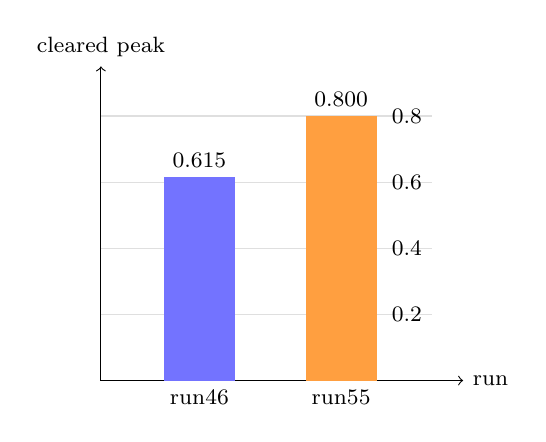
\begin{tikzpicture}[x=1cm,y=4.2cm, every node/.style={font=\footnotesize}]
        \draw[->] (0,0) -- (4.6,0) node[right]{run};
        \draw[->] (0,0) -- (0,0.95) node[above]{cleared peak};
        \foreach \y/\label in {0.2/0.2,0.4/0.4,0.6/0.6,0.8/0.8}
            \draw[gray!25] (0,\y) -- (4.2,\y) node[left, black]{\label};
        \fill[blue!55] (0.8,0) rectangle (1.7,0.615);
        \fill[orange!75] (2.6,0) rectangle (3.5,0.800);
        \node[below] at (1.25,0){run46};
        \node[below] at (3.05,0){run55};
        \node[above] at (1.25,0.615){0.615};
        \node[above] at (3.05,0.800){0.800};
    \end{tikzpicture}
    \caption{Run55 tăng peak cleared rate, nhưng reward mean không so trực tiếp do đổi thang reward}
    \label{fig:reward_v2_clear_peak}
\end{figure}

\section{Entropy plateau}

Một hiện tượng nhất quán xuyên suốt các run là entropy của policy gần như không giảm khỏi vùng 4.40 nat. Với entropy cực đại lý thuyết $H_{\max}\approx 5.49$ nat ở phương trình~\ref{eq:max_entropy}, mức 4.40 tương đương khoảng 80\% của cực đại. Do action mask có thể làm cực đại thực tế thấp hơn, không nên diễn giải đây là policy hoàn toàn ngẫu nhiên; tuy vậy, policy vẫn giữ mức stochastic cao.

\begin{figure}[H]
    \centering
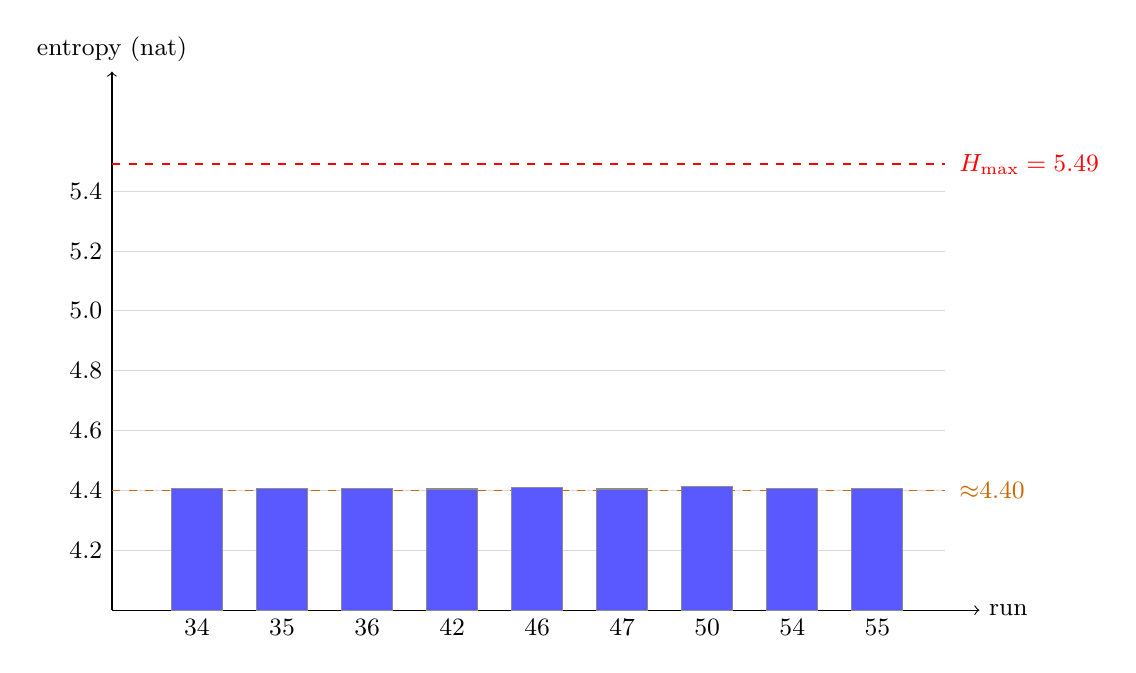
\begin{tikzpicture}[x=1.08cm, y=3.8cm, every node/.style={font=\small}]
        % Grid lines (vẽ trước để bars nằm trên)
        \foreach \y/\lbl in {4.2/4.2, 4.4/4.4, 4.6/4.6, 4.8/4.8, 5.0/5.0, 5.2/5.2, 5.4/5.4}
            \draw[gray!30] (0,\y) node[left, black]{\lbl} -- (9.8,\y);
        % Axes
        \draw[->] (0,4.0) -- (10.2,4.0) node[right]{run};
        \draw[->] (0,4.0) -- (0,5.80) node[above]{entropy (nat)};
        % Đường tham chiếu entropy cực đại lý thuyết
        \draw[dashed, red, thick] (0,5.49) -- (9.8,5.49);
        \node[red, anchor=west] at (9.85,5.49){$H_{\max}=5.49$};
        % Đường tham chiếu vùng bão hòa
        \draw[dashed, orange!80!black] (0,4.40) -- (9.8,4.40);
        \node[orange!80!black, anchor=west] at (9.85,4.40){${\approx}4.40$};
        % Bars (fill + border + run label)
        \fill[blue!65] (0.7,4.0) rectangle (1.3,4.408); \draw[black!45, thin] (0.7,4.0) rectangle (1.3,4.408); \node[below] at (1.0,4.0){34};
        \fill[blue!65] (1.7,4.0) rectangle (2.3,4.407); \draw[black!45, thin] (1.7,4.0) rectangle (2.3,4.407); \node[below] at (2.0,4.0){35};
        \fill[blue!65] (2.7,4.0) rectangle (3.3,4.406); \draw[black!45, thin] (2.7,4.0) rectangle (3.3,4.406); \node[below] at (3.0,4.0){36};
        \fill[blue!65] (3.7,4.0) rectangle (4.3,4.405); \draw[black!45, thin] (3.7,4.0) rectangle (4.3,4.405); \node[below] at (4.0,4.0){42};
        \fill[blue!65] (4.7,4.0) rectangle (5.3,4.409); \draw[black!45, thin] (4.7,4.0) rectangle (5.3,4.409); \node[below] at (5.0,4.0){46};
        \fill[blue!65] (5.7,4.0) rectangle (6.3,4.405); \draw[black!45, thin] (5.7,4.0) rectangle (6.3,4.405); \node[below] at (6.0,4.0){47};
        \fill[blue!65] (6.7,4.0) rectangle (7.3,4.412); \draw[black!45, thin] (6.7,4.0) rectangle (7.3,4.412); \node[below] at (7.0,4.0){50};
        \fill[blue!65] (7.7,4.0) rectangle (8.3,4.407); \draw[black!45, thin] (7.7,4.0) rectangle (8.3,4.407); \node[below] at (8.0,4.0){54};
        \fill[blue!65] (8.7,4.0) rectangle (9.3,4.408); \draw[black!45, thin] (8.7,4.0) rectangle (9.3,4.408); \node[below] at (9.0,4.0){55};
    \end{tikzpicture}
    \caption{Entropy tail-50 của các run chính đều nằm quanh 4.40 nat (${\approx}80\%$ của $H_{\max}$)}
    \label{fig:entropy_plateau}
\end{figure}

Trong phạm vi các ablation đã thử, plateau này không được giải quyết bởi ICM, RND, LSTM, curriculum, beta/aggressive variants, giảm phương sai spawn hoặc reward redesign. Kết luận thận trọng là: entropy plateau là giới hạn thực nghiệm quan sát được trong thiết kế action space và môi trường hiện tại, chưa phải một định lý về PPO. Hướng tiếp theo hợp lý là đơn giản hóa action space, gom bớt branch hoặc thêm inductive bias cho ngắm và né đạn.

\section{Tổng hợp kết quả}

\begin{table}[H]
    \centering
    \scriptsize
    \setlength{\tabcolsep}{3pt}
    \renewcommand{\arraystretch}{1.18}
    \caption{Tổng hợp các run chính}
    \label{tab:master_ablation}
    \begin{tabular}{|>{\raggedright\arraybackslash}p{1.15cm}|>{\raggedright\arraybackslash}p{2.65cm}|>{\centering\arraybackslash}p{1.05cm}|>{\centering\arraybackslash}p{1.95cm}|>{\centering\arraybackslash}p{1.35cm}|>{\raggedright\arraybackslash}p{4.65cm}|}
        \hline
        \textbf{Run} & \textbf{Thiết lập} & \textbf{Steps} & \textbf{Reward} & \textbf{Kills} & \textbf{Kết luận} \\
        \hline
        run34 & PPO baseline & 1.0M & 2.073 & 0.721 & Mốc so sánh; học được chiến đấu cơ bản nhưng trần thấp. \\
        \hline
        run35 & PPO + ICM & 1.0M & 2.416 & 0.752 & Cải thiện nhỏ; inverse loss cao. \\
        \hline
        run36 & PPO + RND & 1.0M & 2.487 & 0.796 & Tốt hơn ICM nhẹ, nhưng chưa tạo thay đổi nổi bật. \\
        \hline
        run42 & PPO + LSTM & 1.0M & 2.411 & 0.769 & Học chậm nhưng tăng dần; lợi ích hạn chế. \\
        \hline
        run46 & PPO + Curriculum & 3.0M & 3.843 & 0.994 & Cải thiện chính, kill/episode và clear rate đều tăng rõ. \\
        \hline
        run47 & Curriculum + LSTM & 3.0M & 3.765 & 0.921 & Không cộng hưởng rõ với curriculum. \\
        \hline
        run50 & Curriculum + ICM & 3.0M & 4.369 & 1.016 & Cộng hưởng nhẹ với curriculum; inverse loss vẫn cao. \\
        \hline
        run54 & 4-tier fixed-to-random & 3.0M & 3.925 & 0.945 & Tương đương run46; fixed-to-random chỉ cải thiện nhẹ. \\
        \hline
        run55 & Curriculum + reward v2 & 3.0M & 9.337 & 1.014 & Clear peak cao hơn; reward scale khác nên không so mean trực tiếp. \\
        \hline
    \end{tabular}
\end{table}

Một lưu ý quan trọng khi đọc Bảng~\ref{tab:master_ablation} là ngân sách huấn luyện giữa các nhóm chưa hoàn toàn đồng nhất. Các run không dùng curriculum như run34, run35, run36 và run42 kết thúc ở 1.0M bước, trong khi các run curriculum chính được huấn luyện đến 3.0M bước. Vì vậy, so sánh giữa hai nhóm phản ánh xu hướng thực nghiệm của toàn bộ cấu hình huấn luyện, nhưng chưa tách biệt hoàn toàn ảnh hưởng của curriculum khỏi ảnh hưởng của thời lượng huấn luyện dài hơn. Để so sánh chặt chẽ hơn, các cấu hình baseline/ICM/RND/LSTM cần được kéo dài lên 3.0M bước, hoặc các run curriculum cần được báo cáo thêm tại cùng mốc 1.0M bước.

\begin{figure}[H]
\centering
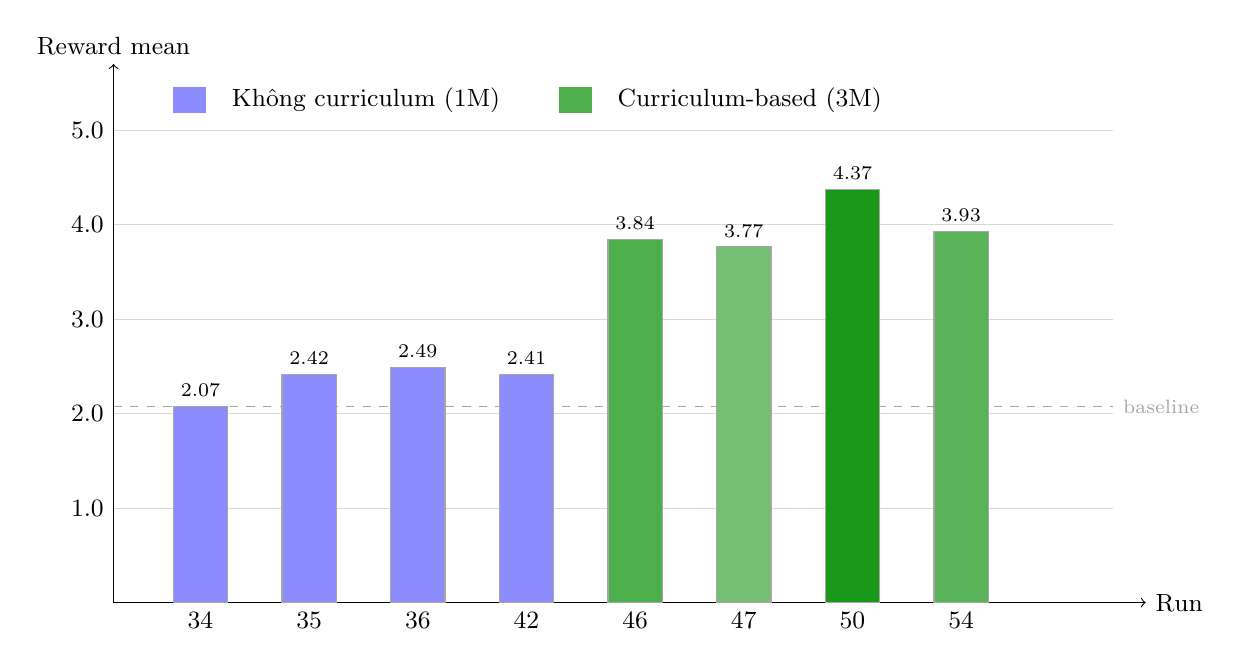
\begin{tikzpicture}[x=1.38cm, y=1.2cm, every node/.style={font=\small}]
  % Axes
  \draw[->] (0,0) -- (9.5,0) node[right]{Run};
  \draw[->] (0,0) -- (0,5.7) node[above]{Reward mean};
  % Grid
  \foreach \y/\lbl in {1/1.0, 2/2.0, 3/3.0, 4/4.0, 5/5.0}
    \draw[gray!30] (0,\y) node[left,black]{\lbl} -- (9.2,\y);
  % Baseline dashed line
  \draw[dashed, gray!70] (0,2.073) -- (9.2,2.073);
  \node[gray!70, anchor=west, font=\scriptsize] at (9.2,2.073){baseline};
  % Bars (no-curriculum: blue; curriculum-based: green)
  \fill[blue!45]          (0.55,0) rectangle (1.05,2.073); \draw[black!35,thin] (0.55,0) rectangle (1.05,2.073); \node[below] at (0.80,0){34}; \node[above,font=\scriptsize] at (0.80,2.073){2.07};
  \fill[blue!45]          (1.55,0) rectangle (2.05,2.416); \draw[black!35,thin] (1.55,0) rectangle (2.05,2.416); \node[below] at (1.80,0){35}; \node[above,font=\scriptsize] at (1.80,2.416){2.42};
  \fill[blue!45]          (2.55,0) rectangle (3.05,2.487); \draw[black!35,thin] (2.55,0) rectangle (3.05,2.487); \node[below] at (2.80,0){36}; \node[above,font=\scriptsize] at (2.80,2.487){2.49};
  \fill[blue!45]          (3.55,0) rectangle (4.05,2.411); \draw[black!35,thin] (3.55,0) rectangle (4.05,2.411); \node[below] at (3.80,0){42}; \node[above,font=\scriptsize] at (3.80,2.411){2.41};
  \fill[green!55!black!70](4.55,0) rectangle (5.05,3.843); \draw[black!35,thin] (4.55,0) rectangle (5.05,3.843); \node[below] at (4.80,0){46}; \node[above,font=\scriptsize] at (4.80,3.843){3.84};
  \fill[green!55!black!55](5.55,0) rectangle (6.05,3.765); \draw[black!35,thin] (5.55,0) rectangle (6.05,3.765); \node[below] at (5.80,0){47}; \node[above,font=\scriptsize] at (5.80,3.765){3.77};
  \fill[green!55!black!90](6.55,0) rectangle (7.05,4.369); \draw[black!35,thin] (6.55,0) rectangle (7.05,4.369); \node[below] at (6.80,0){50}; \node[above,font=\scriptsize] at (6.80,4.369){4.37};
  \fill[green!55!black!65](7.55,0) rectangle (8.05,3.925); \draw[black!35,thin] (7.55,0) rectangle (8.05,3.925); \node[below] at (7.80,0){54}; \node[above,font=\scriptsize] at (7.80,3.925){3.93};
  % Legend
  \fill[blue!45]          (0.55,5.18) rectangle (0.85,5.46); \node[anchor=west] at (1.00,5.32){Không curriculum (1M)};
  \fill[green!55!black!70](4.10,5.18) rectangle (4.40,5.46); \node[anchor=west] at (4.55,5.32){Curriculum-based (3M)};
\end{tikzpicture}
\caption{So sánh reward mean giữa các run dùng reward v1. Đường đứt khoảng ở 2.07 là mức baseline. Run55 (reward v2, mean 9.337) có thang reward khác nên không đưa vào biểu đồ.}
\label{fig:reward_comparison_all}
\end{figure}

\begin{figure}[H]
    \centering
    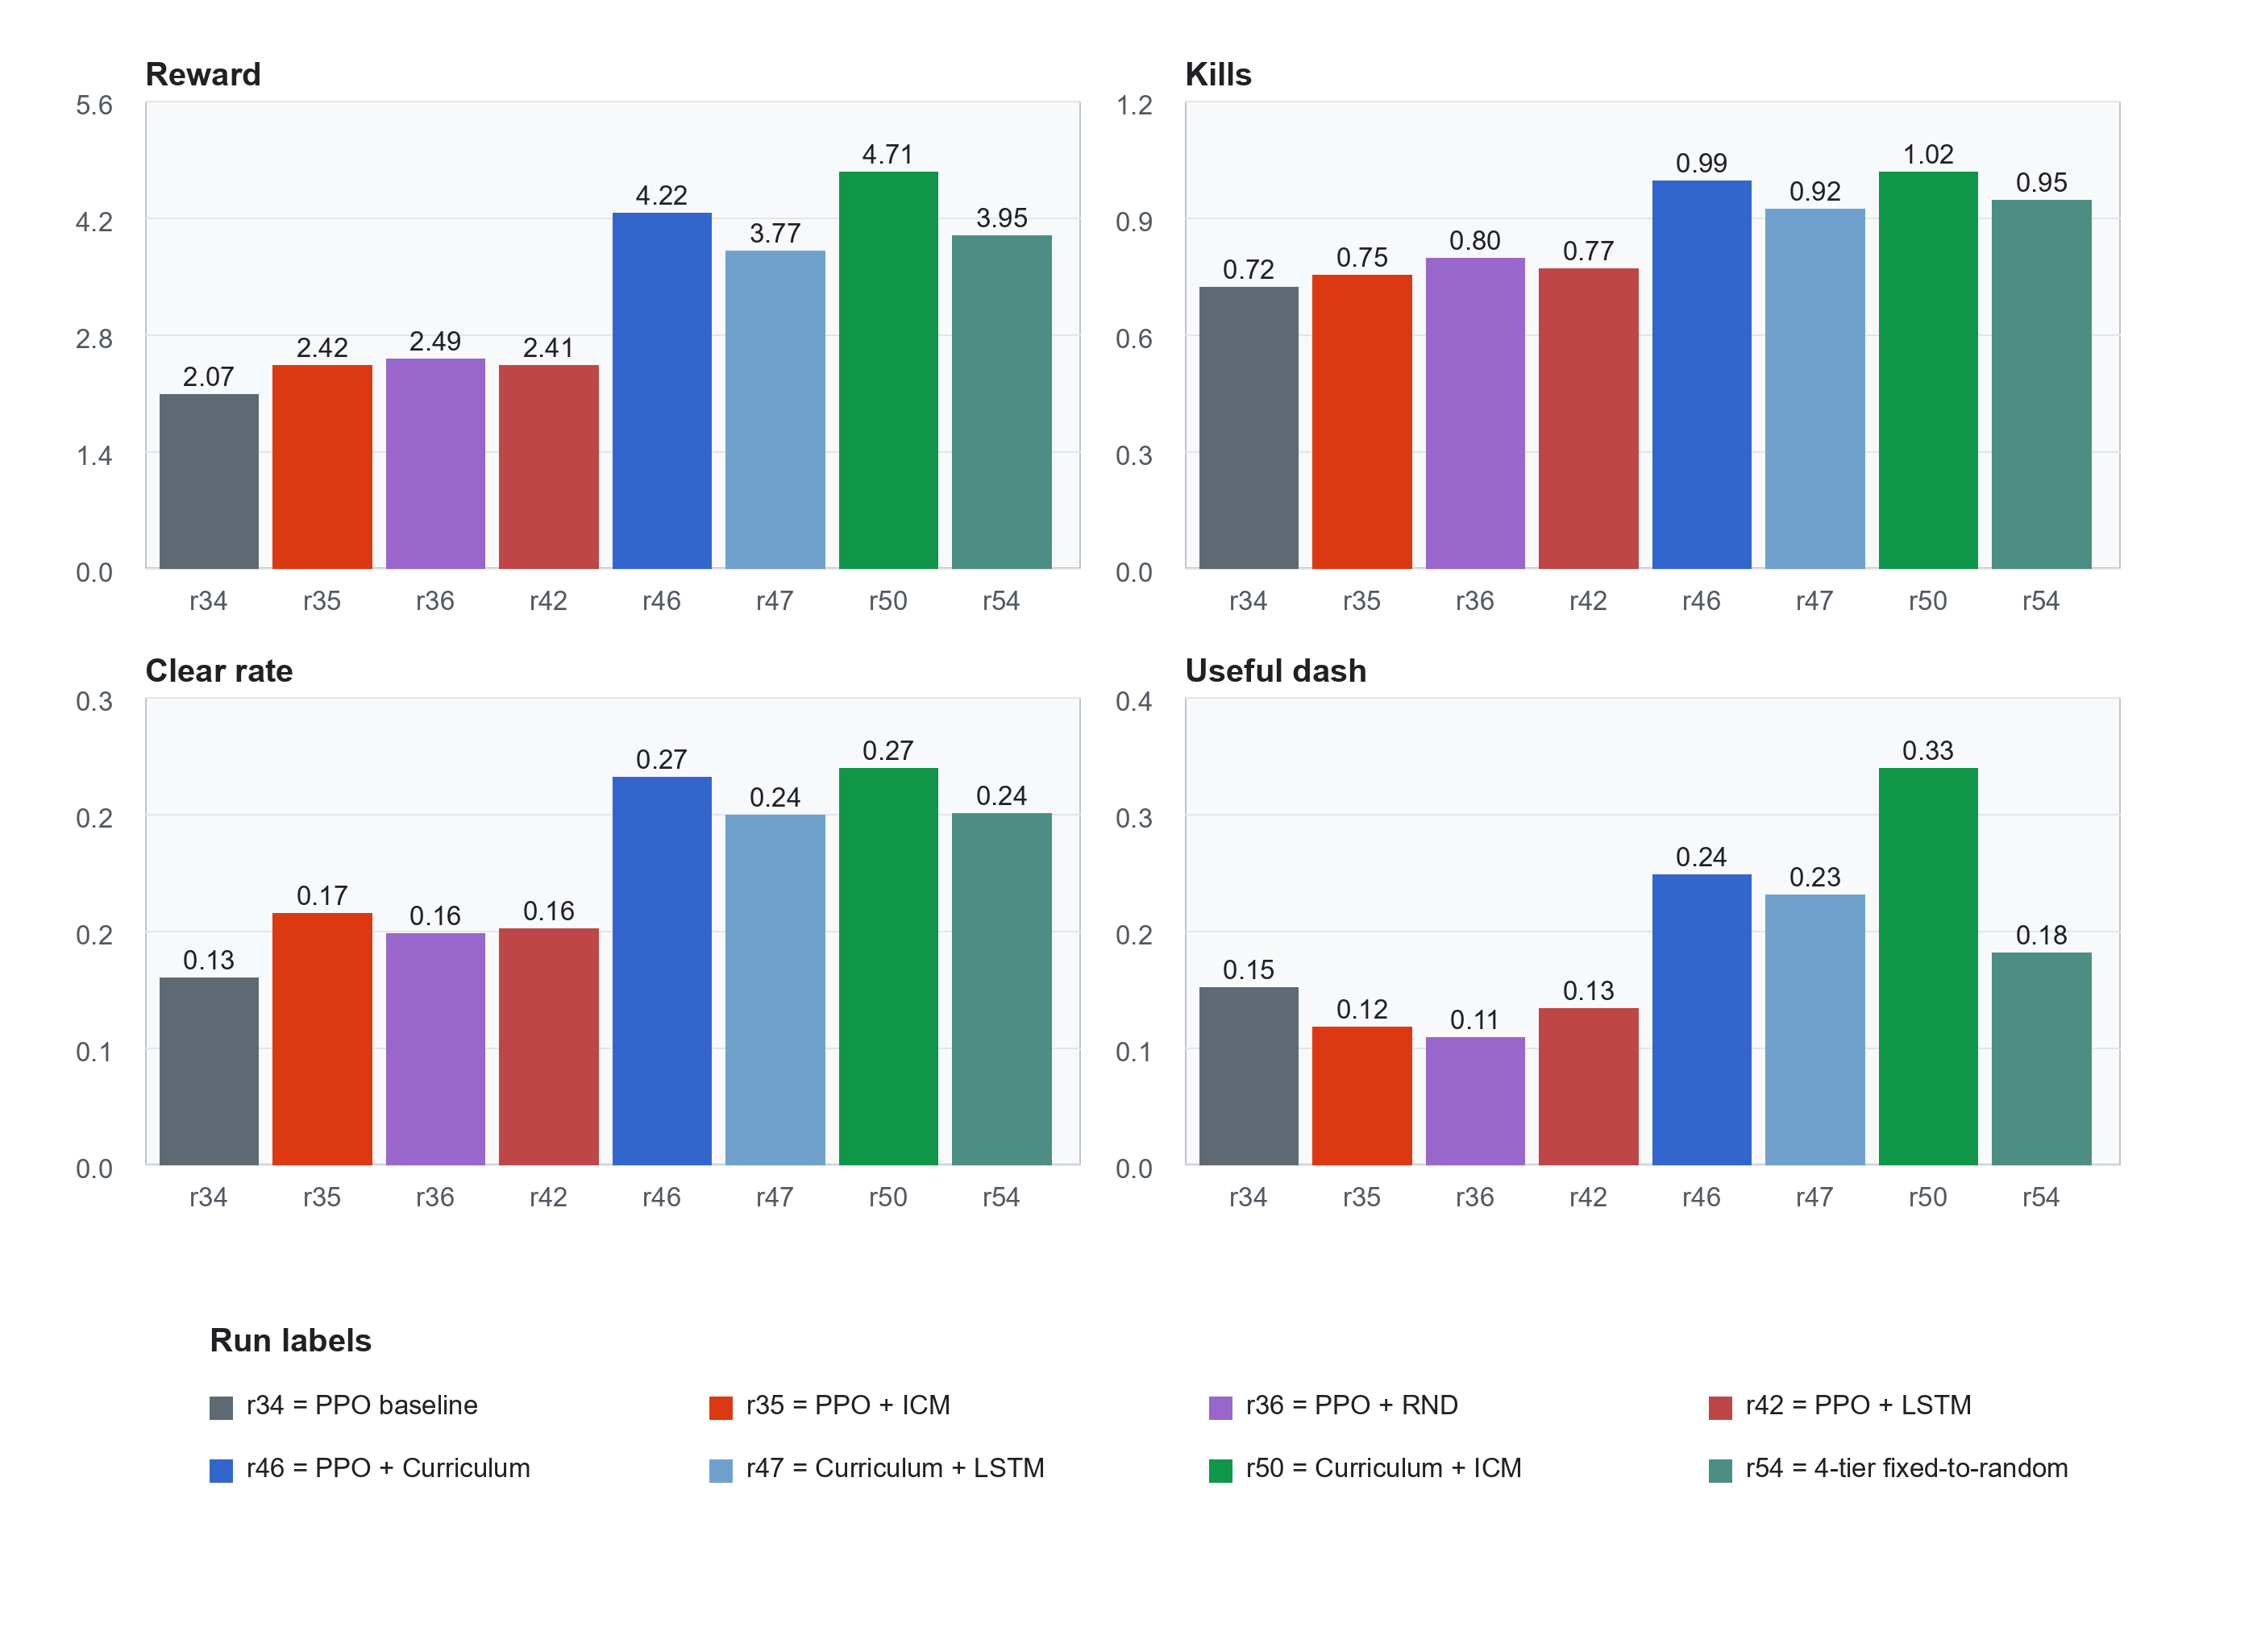
\includegraphics[width=0.98\textwidth]{figures/training/final_metrics_comparison.png}
    \caption{So sánh các chỉ số hành vi cuối run. Hình này bổ sung cho Bảng~\ref{tab:run_metrics_main} bằng cách cho thấy curriculum không chỉ tăng reward mà còn cải thiện số enemy bị tiêu diệt, tỷ lệ dọn phòng và tỷ lệ dash hữu ích.}
    \label{fig:final_metrics_comparison}
\end{figure}

Từ bảng tổng hợp, bốn nhận xét chính được rút ra trong phạm vi thí nghiệm một seed. Thứ nhất, PPO baseline đạt hành vi hợp lý nhưng bị giới hạn ở mức reward khoảng 2.1--2.5. Thứ hai, intrinsic motivation và LSTM chưa tạo cải thiện lớn khi chạy độc lập. Thứ ba, curriculum learning là yếu tố nổi bật nhất; khi kết hợp thêm ICM, reward Hard tăng lên 4.369 nhưng inverse loss vẫn cao. Thứ tư, entropy plateau vẫn tồn tại trong hầu hết cấu hình, cho thấy cần nghiên cứu thêm về action space và cấu trúc policy.
